\chapter{Calculus with Polar Coordinates}

We have been working in Cartesian coordinates, which are rectangular, with $x$ 
representing the horizontal position and $y$ representing the vertical 
position. As we have talked about, you can use polar coordinates to represent circular points. To reviewm another way to represent a position in $2D$ space is with \textbf{
polar coordinates}\index{polar coordinates}. The 
first number and dependent variable is $r$, which represents how 
far the point is from the origin. The second number is $\theta$, which represents the degrees 
of rotation from the the $x$ axis (see Figure-\ref{fig:polarex}). 

\begin{figure}[htbp]
\centering
    \begin{tikzpicture}
	\begin{polaraxis}[xtick = {0,0,deg((pi)/6),deg((2*pi)/6),deg((3*pi)/6),
	deg(4*pi)/6,deg((5*pi)/6), deg((6*pi)/6), deg((7*pi)/6), deg((8*pi)/6), 
	deg((9*pi)/6), deg((10*pi)/6), deg((11*pi)/6)}, xticklabels={,0,
	$\frac{\pi}{6}$,$\frac{\pi}{3}$,$\frac{\pi}{2}$,$\frac{2\pi}{3}$, 
	$\frac{5\pi}{6}$, $\pi$,$\frac{7\pi}{6}$, $\frac{4\pi}{3}$, 
	$\frac{3\pi}{2}$, $\frac{5\pi}{3}$, $\frac{11\pi}{6}$}, ymax = 2.25, clip = false]
		\addplot[white, thick, domain = 0:360, samples = 200]{2.25};
        \addplot[blue, only marks]coordinates {(0,1) (60, 1.5) (240, 2)};
        \addplot[red, domain = 0:60]{1.5};
        \draw[red, -latex](58, 1.5)--(60,1.5);
        \node[] at (65, 1.6) {$(1.5, \frac{\pi}{3})$};
        \node[] at (-15, 1) {$(1, 0)$};
        \addplot[red, domain = -120:0]{2};
        \draw[red, -latex](-118, 2) -- (-120,2);
        \node[] at (-120, 1.8) {$(2, -\frac{5\pi}{6})$};
        \end{polaraxis}
    \end{tikzpicture}
    \caption{Polar coordinates give a degree of rotation, $\theta$, and a 
    distance from the origin, $r$, in the form of $(r, \theta)$}
    \label{fig:polarex}
    \end{figure}

\section{Derivatives of Polar Functions}
Consider the cardioid $r = 2 + \sin{\theta}$ (see Figure~\ref{fig:cardioid}). What 
is the slope of the line tangent to the curve at $\theta = \frac{\pi}{2}$? 

\begin{figure}[htbp]
\centering
    \begin{tikzpicture}
	\begin{polaraxis}[xtick = {0,0,deg((pi)/6),deg((2*pi)/6),deg((3*pi)/6),
	deg(4*pi)/6,deg((5*pi)/6), deg((6*pi)/6), deg((7*pi)/6), deg((8*pi)/6), 
	deg((9*pi)/6), deg((10*pi)/6), deg((11*pi)/6)}, xticklabels={,0,
	$\frac{\pi}{6}$,$\frac{\pi}{3}$,$\frac{\pi}{2}$,$\frac{2\pi}{3}$, 
	$\frac{5\pi}{6}$, $\pi$,$\frac{7\pi}{6}$, $\frac{4\pi}{3}$, $\frac{3\pi}{2}$, 
	$\frac{5\pi}{3}$, $\frac{11\pi}{6}$}, ymax = 2.25, clip = false]
		\addplot[white, thick, domain = 0:360, samples = 200]{2.25};
        \addplot[blue, thick, domain = 0:360, samples = 100]{1 + sin(x)};
        \end{polaraxis}
    \end{tikzpicture}
    \caption{$r = 2 + \sin{\theta}$}
    \label{fig:cardioid}
    \end{figure}

From a visual inspection, we can guess that the slope of the tangent line is 
zero. Let's prove this mathematically:

First, recall that to convert polar coordinates to Cartesian coordinates, we 
can use the trigonometric identities:
$$x = r\cos{\theta}$$
$$y = r\sin{\theta}$$

So, we can write the parametric equation:
$$x = \left[2 + \sin{\theta} \right]\cos{\theta}$$
$$y = \left[ 2 + \sin{\theta} \right]\sin{\theta}$$

Recall from parametric equations that we can use implicit differentiation to 
find $\frac{dy}{dx}$:
$$\frac{dy}{dx} = \frac{\frac{dy}{d\theta}}{\frac{dx}{d\theta}}$$

Finding $\frac{dy}{d\theta}$ and $\frac{dx}{d\theta}$:
$$\frac{dy}{d\theta} = \frac{d}{d\theta} \left( 2\sin{\theta} + \sin^2{\theta} 
\right) = 2\cos{\theta} + 2\sin{\theta}\cos{\theta}$$
$$\frac{dx}{d\theta} = \frac{d}{d\theta} \left( 2\cos{\theta} + \sin{\theta}
\cos{\theta} \right) = \cos^2{\theta} - \sin^2{\theta} - 2\sin{\theta}$$

Substituting $\theta = \frac{\pi}{2}$, we find that:
$$\frac{dy}{d\theta} = 2(0) + 2(1)(0) = 0$$
$$\frac{dx}{d\theta} = (0)^2 - (1)^2 - 2(1) = -3$$

Therefore,
$$\frac{dy}{dx} = \frac{0}{-3} = 0$$

Which is the result we expected from examining the graph of $r = 2 + \sin{
\theta}$. 
\index{polar functions}
\index{polar functions!slope}
So, in general for polar equations, 
\begin{mdframed}[style=important, frametitle={Tangent to a Polar Function}]
For a polar function, $r = f(\theta)$, the slope of a tangent line is given by:
$$\frac{dy}{dx} = \frac{\frac{dy}{d\theta}}{\frac{dx}{d\theta}}$$

Where $y = r \cdot \sin{\theta}$ and $x = r \cdot \cos{\theta}$\footnote{Some textbooks and sources will use a form of this formula that includes the derivatives of $r$ with respect to $\theta$. This book will not focus on this form. }.
\end{mdframed}

\begin{Exercise}[label = polar1]
[This problem was originally presented as a no-calculator, multiple-choice 
question on the 2012 AP Calculus BC exam.] What is the slope of the line 
tangent to the polar curve $r = 1 + 2\sin{\theta}$ at $\theta = 0$?
\vspace{50mm}
\end{Exercise}

\begin{Answer}[ref = polar1]
Recall that for a polar function, $\frac{dy}{dx} = \frac{\frac{dy}{d\theta}}{
\frac{dx}{d\theta}}$. We also know that $x = r \cos{\theta}$, which equals 
$\left[ 1 + 2\sin{\theta} \right] \cdot \cos{\theta} = \cos{\theta} + 2\sin{
\theta}\cos{\theta}$ in this case. We also know that $y = r \cdot \sin{\theta}$, 
which equals $\left[ 1 + 2 \sin{\theta} \right] \cdot \sin{\theta} = \sin{
\theta} + 2 \sin^2{\theta}$ in this case. Taking the derivative with respect 
to $\theta$:
$$\frac{dy}{d\theta} = \frac{d}{d\theta} \left[ \sin{\theta} + 2 \sin^2{\theta} 
\right]$$
$$\frac{dy}{d\theta} = \cos{\theta} + 4\sin{\theta}\cos{\theta}$$

And

$$\frac{dx}{d\theta} = \frac{d}{d\theta} \left[ \cos{\theta} + 2\sin{\theta}\cos{
\theta} \right]$$
$$\frac{dx}{d\theta} = -\sin{\theta} - 2\sin^2{\theta} + 2\cos^2{\theta}$$

Evaluating each at $\theta = 0$:
$$\frac{dy}{d\theta} = \cos{0} + 4\sin{0}\cos{0} = 1 + 0 = 1$$
$$\frac{dx}{d\theta} = -\sin{0} - 2\sin^2{0} + 2\cos^2{0} = 0 - 0 + 2 = 2$$

Therefore, $\frac{dr}{d\theta} = \frac{dy/d\theta}{dx/d\theta} = \frac{1}{2}$
\end{Answer}

\begin{Exercise}[label = polar3]
Find the slope of the tangent line to the given polar curve at the value of 
$\theta$ specified. Use this to write an equation for the tangent line in 
Cartesian coordinates. 
\begin{enumerate}
\item $r = \frac{2}{3}\cos{\theta}$, $\theta = \frac{\pi}{6}$
\item $r = \frac{1}{2\theta}$, $\theta = \frac{\pi}{2}$
\item $r = 2 + 3\cos{\theta}$, $\theta = \frac{2\pi}{3}$
\end{enumerate}
\vspace{120mm}
\end{Exercise}

\begin{Answer}[ref = polar3]
\begin{enumerate}
\item Answer: slope $ = -\frac{\sqrt{3}}{3}$ and an equation for the tangent 
line is $y - \frac{\sqrt{3}}{6} = -\frac{\sqrt{3}}{3} \left( x - \frac{1}{2} 
\right)$. 

Explanation: $\frac{dy}{dx} = \frac{dy/d\theta}{dx/d\theta} = \frac{\frac{d}{d
\theta}r \cdot sin{\theta}}{\frac{d}{d\theta} r \cdot \cos{\theta}} = \frac{
\frac{d}{d\theta} \left( \frac{2}{3} \cos{\theta} \sin{\theta} \right)}{\frac{
d}{d\theta} \left( \frac{2}{3} \cos^2{\theta} \right)} = \frac{\frac{2}{3} 
\left( \cos^2{\theta} -\sin^2{\theta} \right)}{\frac{2}{3} \left( -2\cos{
\theta}\sin{\theta}\right)} = \frac{\sin^2{\theta} - \cos^2{\theta}}{2\cos{
\theta}\sin{\theta}}$

Substituting $\theta = \frac{\pi}{6}$: $\frac{dy}{dx} = \frac{\sin^2{\pi/6} - 
\cos^2{\pi/6}}{2\cos{\pi/6}\sin{\pi/6}} = \frac{\left(1/2 \right)^2 - \left(
\sqrt{3}/2\right)^2}{2\left(\sqrt{3}/2\right) \left(1/2\right)} = \frac{1/4 - 
3/4}{\sqrt{3}/2} = \frac{-1/2}{\sqrt{3}/2} = \frac{-1}{2} \cdot \frac{2}{\sqrt{
3}} = -\frac{\sqrt{3}}{3}$

To write an equation for a line, we need a Cartesian point. First, we find $r$ 
at $\theta = \frac{\pi}{6}$: $r = \frac{2}{3}\cos{\left( \frac{\pi}{6} \right)}
= \frac{2}{3} \cdot \frac{\sqrt{3}}{2} = \frac{\sqrt{3}}{3}$. So the point the 
tangent passes through is the polar coordinate $\left( \frac{\sqrt{3}}{3}, 
\frac{\pi}{6} \right)$. We convert this to Cartesian coordinates: $x = r \cos{
\theta} = \frac{\sqrt{3}}{3} \cdot \cos{\left( \frac{\pi}{6} \right)} = \frac{
\sqrt{3}}{3} \cdot \frac{\sqrt{3}}{2} = \frac{3}{6} = \frac{1}{2}$ And $y = r
\sin{\theta} = \frac{\sqrt{3}}{3} \cdot \sin{\left( \frac{\pi}{6} \right)} = 
\frac{\sqrt{3}}{3} \cdot \frac{1}{2} = \frac{\sqrt{3}}{6}$

So, an equation for a line with slope $-\frac{\sqrt{3}}{3}$ that passes 
through Cartesian coordinate $\left( \frac{1}{2}, \frac{\sqrt{3}}{6} \right)$ 
is: $y - \frac{\sqrt{3}}{6} = -\frac{\sqrt{3}}{3} \left( x - \frac{1}{2} 
\right)$

\item Answer: slope $= \frac{2}{\pi}$ and an equation for the tangent line is 
$y - \frac{1}{\pi} = \frac{2}{\pi}x$

Explanation: $\frac{dy}{dx} = \frac{dy/d\theta}{dx/d\theta} = \frac{\frac{d}{d
\theta} \left( \frac{\sin{\theta}}{2\theta}\right)}{\frac{d}{d\theta} \left( 
\frac{\cos{\theta}}{2\theta}\right)} = \frac{\frac{\theta \cos{\theta} - \sin{
\theta}}{2\theta^2}}{-\frac{\theta\sin{\theta} + \cos{\theta}}{2\theta^2}} = 
\frac{\sin{\theta} - \theta\cos{\theta}}{\theta\sin{\theta} + \cos{\theta}}$. 

Substituting $\theta = \frac{\pi}{2}$: $\frac{dy}{dx} = \frac{\sin{\frac{\pi}{
2}} - \left( \frac{\pi}{2}\right) \cos{\frac{\pi}{2}}}{\left( \frac{\pi}{2} 
\right) \sin{\frac{\pi}{2}} + \cos{\frac{\pi}{2}}} = \frac{1 - \left( \frac{
\pi}{2} \right) \cdot 0 }{\left( \frac{\pi}{2} \right) \cdot 1 + 0} = \frac{1}{
\frac{\pi}{2}} = \frac{2}{\pi}$

To write an equation for a line, we need a Cartesian point. First, we find $r$ 
at $\theta = \frac{\pi}{2}$: $r = \frac{1}{2\theta} = \frac{1}{2\frac{\pi}{2}} 
= \frac{1}{\pi}$. So the tangent line passes through the point with polar 
coordinates $\left( \frac{1}{\pi}, \frac{\pi}{2} \right)$. We convert this to 
Cartesian coordinates: $x = r \cdot \cos{\theta} = \frac{1}{\pi} \cdot \cos{
\frac{\pi}{2}} = \frac{1}{\pi} \cdot 0 = 0$ and $y = r \cdot \sin{\theta} = 
\frac{1}{\pi} \cdot \sin{\frac{\pi}{2}} = \frac{1}{\pi} \cdot 1 = \frac{1}{
\pi}$. 

So, an equation for a line with slope $\frac{2}{\pi}$ that passes through 
Cartesian coordinate $\left( 0, \frac{1}{\pi} \right)$ is $y - \frac{1}{\pi} = 
\frac{2}{\pi} x$

\item Answer: slope $= -\frac{5}{\sqrt{3}}$ and an equation for the tangent 
line is $y - \frac{\sqrt{3}}{4} = \left( -\frac{5}{\sqrt{3}} \right) \left( x 
+ \frac{1}{4} \right)$.

Explanation: $\frac{dy}{dx} = \frac{dy/d\theta}{dx/d\theta} = \frac{\frac{d}{d
\theta} \left[ \left( 2 + 3\cos{\theta}\right) \cdot \sin{\theta} \right]}{
\frac{d}{d\theta} \left[ \left( 2 + 3\cos{\theta} \right) \cdot \cos{\theta} 
\right]} = \frac{\cos{\theta} \left( 2 + 3\cos{\theta}\right) - 3\sin^2{\theta}
}{\left( 2 + 3\cos{\theta}\right) \cdot \left(-\sin{\theta} \right) + \cos{
\theta} \left( -3\sin{\theta} \right)} = \frac{\cos{\theta} \left( 2 + 3\cos{
\theta}\right) - 3\sin^2{\theta}}{-2\sin{\theta} \left( 1 + 3\cos{\theta} 
\right)}$. 

Substituting $\theta = \frac{2\pi}{3}$: $\frac{dy}{dx} = \frac{\cos{\frac{2\pi
}{3}} \left( 2 + 3\cos{\frac{2\pi}{3}}\right) - 3\sin^2{\frac{2\pi}{3}}}{-2
\sin{\frac{2\pi}{3}} \left( 1 + 3\cos{\frac{2\pi}{3}}\right)} = \frac{\left( 
-\frac{1}{2} \right) \left( 2 + 3\left( -\frac{1}{2} \right)\right) - 3\left( 
\frac{\sqrt{3}}{2} \right)^2}{-2\left( \frac{\sqrt{3}}{2} \right) \left( 1 + 3
\left( -\frac{1}{2} \right) \right)} = \frac{\left( -\frac{1}{2}\right) \left(2
- \frac{3}{2} \right) - 3\left( \frac{3}{4} \right)}{-\sqrt{3} \left( 1 - 
\frac{3}{2} \right)} = \frac{\left( -\frac{1}{2}\right) \left( \frac{1}{2}
\right) - \frac{9}{4}}{-\sqrt{3} \left( -\frac{1}{2}\right)} = \frac{-\frac{1}{
4} - \frac{9}{4}}{\frac{\sqrt{3}}{2}} = -\frac{\frac{10}{4}}{\frac{\sqrt{3}}{2
}} = -\frac{10 \cdot 2}{4 \cdot \sqrt{3}} = -\frac{5}{\sqrt{3}}$

To write an equation for a tangent line, we need a Cartesian point. First, we 
find $r$ at $\theta = \frac{2\pi}{3}$: $r = 2 + 3\cos{\frac{2\pi}{3}} = 2 + 3 
\left( \frac{-1}{2}\right) = 2 - \frac{3}{2} = \frac{1}{2}$. So the tangent 
line passes through polar coordinate $\left( \frac{1}{2}, \frac{2\pi}{3} 
\right)$. We convert this to Cartesian coordinates: $x = r \cos{\theta} = 
\frac{1}{2} \cos{\frac{2\pi}{3}} = \frac{1}{2} \left(-\frac{1}{2} \right) = -
\frac{1}{4}$ and $y = r \sin{\theta} = \frac{1}{2} \sin{\frac{2\pi}{3}} = 
\frac{1}{2} \left( \frac{\sqrt{3}}{2}\right) = \frac{\sqrt{3}}{4}$. 

So, an equation with slope $-\frac{\sqrt{5}}{3}$ that passes through the 
Cartesian coordinate $\left( -\frac{1}{4}, \frac{\sqrt{3}}{4}\right)$ is: $y - 
\frac{\sqrt{3}}{4} = \left( -\frac{5}{\sqrt{3}} \right) \left(x + \frac{1}{4} 
\right)$
\end{enumerate}
\end{Answer}

\section{Integrals of Polar Functions}
Similar to Cartesian functions, an integral of a polar function tells us the 
area within the function. We say "within" as opposed to "under" because a 
polar function describes how far from the origin the graph is based on the 
angle. Consider the graph of $r = 2\sin{\theta}$ (figure \ref{fig:2sine}). 
Geometrically, we expect the area inside the curve to be $\pi r^2 = \pi$. 
However, this is not the result we get from directly integrating the function 
(we only integrate from $\theta = 0$ to $\theta = \pi$ because the circle is 
complete when $\theta$ reaches $\pi$): 
$$\int_0^{\pi} 2\sin{\theta}\,d\theta = -2\cos{\theta}|_{\theta = 0}^{\theta 
= \pi}$$
$$= -2 \left[ \cos{\pi} - \cos{0} \right] = -2 \left[ -1 - 1 \right] = 4 \neq 
\pi$$

\begin{figure}[htbp]
\centering
    \begin{tikzpicture}
        \begin{polaraxis}[xtick = {0,0,deg((pi)/6), deg((2*pi)/6), deg((3*pi)/6), 
        deg(4*pi)/6, deg((5*pi)/6), deg((6*pi)/6), deg((7*pi)/6), deg((8*pi)/6), 
        deg((9*pi)/6), deg((10*pi)/6), deg((11*pi)/6)}, xticklabels={,0, $\frac{
        \pi}{6}$, $\frac{\pi}{3}$, $\frac{\pi}{2}$, $\frac{2\pi}{3}$, $\frac{5
        \pi}{6}$, $\pi$, $\frac{7\pi}{6}$, $\frac{4\pi}{3}$, $\frac{3\pi}{2}$,
         $\frac{5\pi}{3}$, $\frac{11\pi}{6}$}, ymax = 2.25, clip = false, xmin 
         = 0, xmax = 180]
            \addplot[blue, thick, domain = 0:360, samples = 100]{2*sin(x)};
            \addplot[white, thick, domain = 0:360, samples = 100]{2.25};
            \addplot[blue, mark=*] coordinates {(90, 1)};
            \draw[black, dashed] (90, 1) -- (135, 1.414);
            \draw[black, |-|] (90, 1.1) -- (130, 1.464);
            \node[] at (110, 1.4) {$r = 1$};
        \end{polaraxis}
    \end{tikzpicture}
    \caption{The graph of $r = 2\sin{\theta}$ is a circle of radius $1$ 
    centered at $(1, \frac{\pi}{2})$}
    \label{fig:2sine}
\end{figure}

Clearly something else is happening here. We can just take the integral of a 
Cartesian function because the area of a rectangle is the base times the 
height. When integrating Cartesian functions, the base is given by the $dx$ 
and the height by the function, $f(x)$. In polar coordinates, the integral 
sweeps across a $\theta$ interval, making a wedge, not a rectangle. 

Let us consider a generic polar function, shown in figure \ref{fig:generic}

\begin{figure}[htbp]
\centering
    \begin{tikzpicture}[scale = 0.75]
        \draw[-latex] (-0.1, 0) -- (10, 0) node[right] {$x$};
        \draw[-latex] (0, -0.1) -- (0, 7) node[above] {$y$};
        \draw[blue, thick] (0, 5.7) 
        to[out = 35, in = 180, looseness = 1.1] (2, 7)
        to[out = 0, in = 135, looseness = 1.15] (3.4, 6)
        to[out = -45, in = 165, looseness = 0.9] (4.2, 5)
        to[out = -15, in = 170, looseness = 1.15] (6, 4.5)
        to[out = 350, in = 130, looseness = 1.2] (7.8, 4)
        to[out = 310, in = 100, looseness = 1.1] (8.5, 3)
        to[out = 280, in = 110, looseness = 1.1] (9, 1.8)
        to[out = 290, in = 135, looseness = 1.1] (10, 0); 
        \draw[black, dashed] (0,0) -- (7.8, 4);
        \node[] at (8.2, 4.2) {$(r$, $\theta)$};
        \draw[red, dashed, -latex] (1,0) arc [start angle = 0, end angle = 22, 
        x radius = 1, y radius = 1.4];
        \node[red] at (1.35, 0.25) {$\theta$};
        \draw[red, dashed, |-|] (0, 0.2) -- (7.8, 4.2);
        \node[red] at (3.9, 2.3) {$r$};
    \end{tikzpicture}
    \caption{A generic polar function}
    \label{fig:generic}
\end{figure}

Suppose we are interested in a specific region, bounded by $a \leq \theta \leq 
b$ (see figure \ref{fig:region}). 

\begin{figure}[htbp]
\centering
    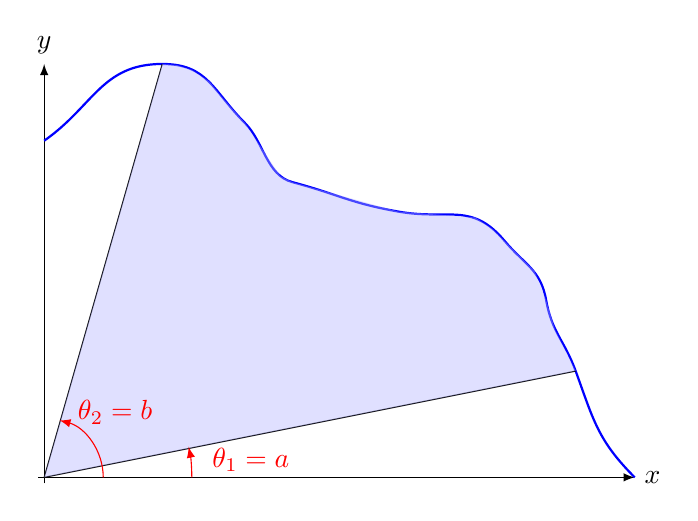
\begin{tikzpicture}[scale = 0.75]
        \draw[-latex] (-0.1, 0) -- (10, 0) node[right] {$x$};
        \draw[-latex] (0, -0.1) -- (0, 7) node[above] {$y$};
        \draw[blue, thick] (0, 5.7) 
        to[out = 35, in = 180, looseness = 1.1] (2, 7)
        to[out = 0, in = 135, looseness = 1.15] (3.4, 6)
        to[out = -45, in = 165, looseness = 0.9] (4.2, 5)
        to[out = -15, in = 170, looseness = 1.15] (6, 4.5)
        to[out = 350, in = 130, looseness = 1.2] (7.8, 4)
        to[out = 310, in = 100, looseness = 1.1] (8.5, 3)
        to[out = 280, in = 110, looseness = 1.1] (9, 1.8)
        to[out = 290, in = 135, looseness = 1.1] (10, 0); 
        \draw[black] (0,0) -- (2, 7);
        \draw[black] (0,0) -- (9, 1.8);
        \fill[blue!30, opacity = 0.4] (0,0) -- (9, 1.8) -- (8.65, 2.5) -- 
        (8.5, 3) --  (8.3, 3.5) -- (7.8, 4) -- (7.6, 4.2) -- (7.3, 4.4) -- 
        (6, 4.5) -- (4.2, 5) -- (4, 5.1) -- (3.4, 6) -- (3, 6.45) -- (2.8, 6.7) 
        -- (2.5, 6.9) -- (2.25, 6.98) -- (2, 7) -- cycle;
        \draw[red, -latex] (1, 0) arc [start angle = 0, end angle = 75, 
        x radius = 1, y radius = 1];
        \node[red] at (1.2, 1.1) {$\theta_2 = b$};
        \draw[red, -latex] (2.5, 0) arc [start angle = 0, end angle = 12, 
        x radius = 2.5, y radius = 2.5];
        \node[red] at (3.5, 0.3) {$\theta_1 = a$};
    \end{tikzpicture}
    \caption{A generic polar with a region from $\theta = a$ to $\theta = b$ 
    highlighted}
    \label{fig:region}
\end{figure}

We can divide the region into many small sectors. Then, each small sector has a 
central angle $\Delta \theta$ and a radius $r(\theta_i^*)$, where $\theta_{i-1}
 < \theta_i^* < \theta_i$ (see figure \ref{fig:onesector}).

\begin{figure}[htbp]
\centering
    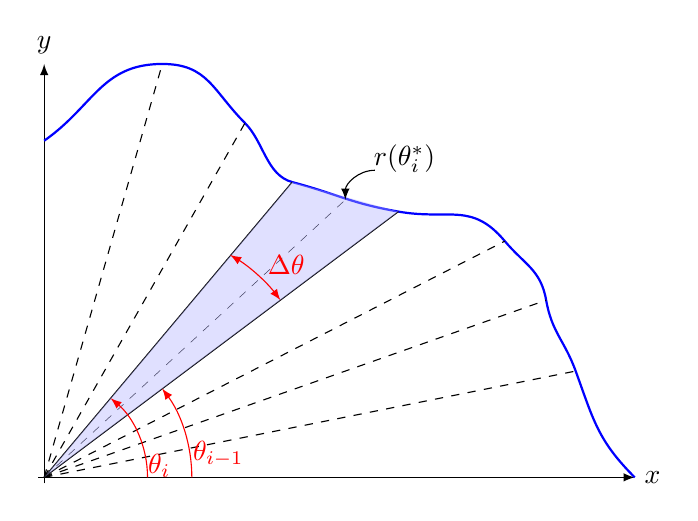
\begin{tikzpicture}[scale = 0.75]
        \draw[-latex] (-0.1, 0) -- (10, 0) node[right] {$x$};
        \draw[-latex] (0, -0.1) -- (0, 7) node[above] {$y$};
        \draw[blue, thick] (0, 5.7) 
        to[out = 35, in = 180, looseness = 1.1] (2, 7)
        to[out = 0, in = 135, looseness = 1.15] (3.4, 6)
        to[out = -45, in = 165, looseness = 0.9] (4.2, 5)
        to[out = -15, in = 170, looseness = 1.15] (6, 4.5)
        to[out = 350, in = 130, looseness = 1.2] (7.8, 4)
        to[out = 310, in = 100, looseness = 1.1] (8.5, 3)
        to[out = 280, in = 110, looseness = 1.1] (9, 1.8)
        to[out = 290, in = 135, looseness = 1.1] (10, 0); 
        \draw[black, dashed] (0,0) -- (2, 7);
        \draw[black, dashed] (0,0) -- (3.4, 6);
        \draw[black] (0,0) -- (4.2, 5);
        \draw[black] (0,0) -- (6, 4.5);
        \draw[black, very thin, dashed](0,0) -- (5.1, 4.7);
        \draw[black, dashed] (0,0) -- (7.8, 4);
        \draw[black, dashed] (0,0) -- (8.5, 3);
        \draw[black, dashed] (0,0) -- (9, 1.8);
        \fill[blue!30, opacity = 0.4](0,0) -- (4.2, 5) -- (6, 4.5) -- cycle;
        \draw[red, -latex] (1.75, 0) arc [start angle = 0, end angle = 50, 
        x radius = 1.75, y radius = 1.75];
        \draw[red, -latex] (2.5, 0) arc [start angle = 0, end angle = 37, 
        x radius = 2.5, y radius = 2.5];
        \node[red] at (1.95, 0.2) {$\theta_i$};
        \node[red] at (2.95, 0.4) {$\theta_{i - 1}$};
        \draw[latex-, black] (5.1, 4.7) arc [start angle = 180, end angle = 90, 
        x radius = 0.5, y radius = 0.5];
        \node[] at (6.1, 5.4) {$r(\theta_i^*)$};
        \draw[red, latex-latex] (4, 3) arc [start angle = 37, end angle = 59, 
        x radius = 3, y radius = 3];
        \node[red] at (4.1, 3.6) {$\Delta \theta$};
    \end{tikzpicture}
    \caption{A single sector from $\theta_{i-1}$ to $\theta_i$}
    \label{fig:onesector}
\end{figure}

What is the area of the $i^{th}$ sector? Recall from the chapter on circles 
that the area of a sector with angle $\theta$ and length $r$ is $A = \frac{1}{2
} r^2 \theta$. Substituting, we see the area of the $i^{th}$ sector is:
$$A_i = \frac{1}{2} \left[ r(\theta_i^*) \right]^2 d\theta$$

Therefore, the total area of the whole sector from $\theta = a$ to $\theta 
= b$ is the limit as the number of sectors approaches infinity of sum of the 
areas of all the small sectors:
$$A = \lim_{n \to \infty} \sum_{i = 1}^n \frac{1}{2} \left[ r( \theta_i^*) 
\right] ^2 \Delta \theta$$

Does this look familiar? It is the definition of an integral!
$$\lim_{n \to \infty} \sum_{i = 1}^n \frac{1}{2} \left[ r( \theta_i^*) \right] 
^2 \Delta \theta = \int_a^b \frac{1}{2} \left[ r(\theta) \right]^2\,d\theta$$

\begin{mdframed}[style=important, frametitle={Area of a Polar Function}]
The area of a polar function is given by the integral 
$$\int_a^b \frac{1}{2} r^2\,d\theta$$

Where $r$ is a function of $\theta$. 
\end{mdframed}

We can check this with the example from the beginning of the section. Recall 
that the polar function $r =  2\sin{\theta}$ graphs a circle with a radius of 
1. Therefore, we expect the area enclosed by the graph of $r = 2\sin{\theta}$ 
from $\theta = 0$ to $\theta = \pi$ to be $\pi$:
$$A = \frac{1}{2} \int_0^{\pi} \left[ 2\sin{\theta} \right]^2\,d\theta$$
$$A = 2 \int_0^{\pi} \sin^2{\theta}\,d\theta = 2 \int_0^{\pi} \left[ \frac{1 - 
\cos{2\theta}}{2} \right]\,d\theta$$
$$A = \int_0^{\pi} \left[ 1 - \cos{2\theta} \right]\,d\theta = \left[\theta - 
\frac{1}{2}\sin{2\theta} \right]_{\theta = 0}^{\theta = \pi}$$
$$A = \left[\pi - 0 \right] - \left[0 - 0 \right] = \pi$$

Which is the expected result, confirming our formula for the area within a 
polar function. 

\textbf{Example}: The graph of $r = 3\sin{2\theta}$ is shown below. What is 
the total area enclosed by the graph?

\begin{figure}[htbp]
\centering
    \begin{tikzpicture}
        \begin{polaraxis}[xtick = {0,0,deg((pi)/6), deg((2*pi)/6), deg((3*pi)/6), 
        deg(4*pi)/6, deg((5*pi)/6), deg((6*pi)/6), deg((7*pi)/6), deg((8*pi)/6), 
        deg((9*pi)/6), deg((10*pi)/6), deg((11*pi)/6)}, xticklabels={,0, $\frac{
        \pi}{6}$, $\frac{\pi}{3}$, $\frac{\pi}{2}$, $\frac{2\pi}{3}$, $\frac{5
        \pi}{6}$, $\pi$, $\frac{7\pi}{6}$, $\frac{4\pi}{3}$, $\frac{3\pi}{2}$, 
        $\frac{5\pi}{3}$, $\frac{11\pi}{6}$}, ymax = 3.25, clip = false, xmin = 0, 
        xmax = 360]
            \addplot[blue, thick, domain = 0:360, samples = 150]{3*sin(2*x)};
            \addplot[white, thick, domain = 0:360, samples = 100]{3.25};
        \end{polaraxis}
    \end{tikzpicture}
    \caption{$r = 3\sin{2\theta}$}
    \label{fig:fourlobe}
\end{figure}

\textbf{Solution}: Since each lobe is symmetric to the others, we can find the 
area of one lobe and multiply it by four. To find the area of one lobe, we 
need to determine an interval for $\theta$ that defines one lobe. You can 
imagine each lobe being draw out from the center and then back in. So, we will 
find where $r = 0$:
$$0 = 3\sin{2\theta}$$
$$\sin{2\theta} = 0$$
$$2\theta = n\pi$$
$$\theta = \frac{n\pi}{2}$$

Taking the first two solutions, $\theta = 0$ and $\theta = \frac{\pi}{2}$, as our 
limits of integration, we see that the area of one lobe is:
$$A_{lobe} = \frac{1}{2} \int_0^{\pi/2} \left[3 \sin{2 \theta} \right]^2\,d
\theta$$
$$A_{lobe} = \frac{9}{2} \int_0^{\pi/2} \sin^2{2\theta}\,d\theta$$

Applying the half-angle formula $\sin^2{\theta} = \frac{1 - \cos{2\theta}}{2}$, 
we see that:
$$A_{lobe} = \frac{9}{2} \int_0^{\pi/2} \frac{1 - \cos{4\theta}}{2}\,d\theta = 
\frac{9}{4} \int_0^{\pi / 2} 1 - \cos{4\theta} \, d\theta$$
$$= \frac{9}{4} \left[ \theta - \frac{1}{4} \sin{4\theta} \right]_{\theta = 0}^
{\theta = \pi / 2} = \frac{9}{4} \left( \frac{\pi}{2} - 0 \right) - \frac{9}{4}
\left( \frac{1}{4} \right) \left( \sin{2\pi} - \sin{0} \right)$$
$$= \frac{9\pi}{8} - \frac{9}{16} \left( 0 \right) = \frac{9\pi}{8}$$

Since the area of one lobe is $\frac{9\pi}{8}$, the area of all four lobes is 
$\frac{9\pi}{2}$.

\subsection{Area between polar curves}
Consider the circle $r = 6\sin{\theta}$ and the cardioid $r = 2 + 2\sin{\theta}
$. How can we find the area that lies inside the circle, but outside the 
cardioid (see figure \ref{fig:twocurves})? First, let's find where these curves
intersect. This will determine the limits of any integrals we take.
$$6\sin{\theta} = 2 + 2\sin{\theta}$$
$$3\sin{\theta} = 1 = \sin{\theta}$$
$$2\sin{\theta} = 1$$
$$\sin{\theta} = \frac{1}{2}$$
$$\theta = \frac{\pi}{6}, \frac{5\pi}{6}$$

\begin{figure}[htbp]
	\centering
    \begin{tikzpicture}
        \begin{polaraxis}[xtick = {0, 30, 60, 90, 120, 150, 180, 210, 240, 
        270, 300, 330}, xticklabels = {$0$, $\frac{\pi}{6}$, $\frac{\pi}{3}$, 
        $\frac{\pi}{2}$, $\frac{2\pi}{3}$, $\frac{5\pi}{6}$, $\pi$, 
        $\frac{7\pi}{6}$, $\frac{4\pi}{3}$, $\frac{3\pi}{2}$, $\frac{5\pi}{3}$,
        $\frac{11\pi}{6}$}, ymax = 6.25, clip = false]
            \addplot[white, very thick, domain = 0:360, samples = 200]{6.25};
            \addplot[black, thick, domain = 0:180, samples =100]{6*sin(x)};
            \addplot[blue, thick, domain = 0:360, samples = 100]{2 + 2*sin(x)};
            \fill[blue!30, opacity = 0.4] (30, 3) -- (40, 3.86) -- (50, 4.60) 
            -- (60, 5.20) -- (70, 5.64) -- (80, 5.91) -- (90, 6) -- (100, 5.91)
            -- (110, 5.64) -- (120, 5.20) -- (130, 4.6) -- (140, 3.86) -- 
            (150, 3) -- (140, 3.29) -- (130, 3.53) -- (120, 3.73) -- 
            (110, 3.88) -- (100, 3.97) -- (90, 4) -- (80, 3.97) -- (70, 3.88) 
            -- (60, 3.73) -- (50, 3.53) -- (40, 3.29) -- cycle;
        \end{polaraxis}
    \end{tikzpicture}
    \caption{The area inside $r = 6\sin{\theta}$ and outside of $r = 2 + 2\sin{
    \theta}$ is highlighted}
    \label{fig:twocurves}
\end{figure}

Recall that for Cartesian functions, to find the area between two curves, we 
subtract the area under the lower curve from the total area under the higher 
curve. In polar coordinates, we want to subtract the area in the inner curve 
from the total area in the outer curve. In this case, the outer curve is $r = 
6\sin{\theta}$ and the inner curve is $r = 2 + 2\sin{\theta}$. We have already 
found our limits of integration ($\frac{\pi}{6} \leq \theta \leq \frac{5 \pi}{
6}$), so we set up and evaluate our integral:
$$A_{between} = \frac{1}{2} \int_{\pi / 6}^{5 \pi / 6} \left[ 4 \sin{\theta} 
\right]^2\,d\theta - \frac{1}{2} \int_{\pi / 6}^{5 \pi / 6} \left[ 2 + 2 \sin{
\theta} \right]^2\,d\theta$$
$$= \frac{1}{2} \int_{\pi / 6}^{5 \pi / 6} \left[ 16 sin^2{\theta} - 4 - 8 
\sin{\theta} - 4 \sin^2{\theta} \right] \, d\theta$$
$$= \int_{\pi / 6}^{5 \pi / 6} \left[ 6 \sin^2{\theta} - 4\sin{\theta} - 2 
\right]\, d\theta$$
$$= \int_{\pi / 6}^{5 \pi / 6} \left[ 3 \left( 1 - \cos{2\theta} \right) - 4
\sin{\theta} - 2 \right] \, d\theta$$
$$= \int_{\pi / 6}^{5 \pi / 6} \left[ 1 - 3\cos{2\theta} - 4\sin{\theta} 
\right] \, d\theta$$
$$= \left[ \theta - \frac{3}{2}\sin{2\theta} + 4\cos{\theta} \right]_{\theta = 
\pi / 6}^{\theta = 5 \pi / 6}$$
$$= \left[ \frac{5\pi}{6} - \frac{\pi}{6} \right] - \left[ \frac{3}{2} \sin{
\left( 2 \cdot \frac{5\pi}{6} \right)} - \frac{3}{2} \sin{\left( 2 \cdot \frac{
\pi}{6} \right)} \right] + \left[ 4\cos{\frac{5\pi}{6}} - 4\cos{\frac{\pi}{6}} 
\right]$$
$$= \frac{4\pi}{6} - \left[ \frac{3}{2} \cdot -\frac{\sqrt{3}}{2} - \frac{3}{2}
\cdot \frac{\sqrt{3}}{2} \right] + \left[ 4 \cdot -\frac{\sqrt{3}}{2} - 4 \cdot
\frac{\sqrt{3}}{2} \right]$$
$$= \frac{2\pi}{3} + \frac{3\sqrt{3}}{2} - 4\sqrt{3} = \frac{2\pi}{3} + \frac{3
\sqrt{3} - 8\sqrt{3}}{2} = \frac{2\pi}{3} - \frac{5\sqrt{3}}{2}$$

(\textit{Note}: Because these polar functions are symmetric about the $y$-axis,
we could have also taken the integral from $\theta = \frac{\pi}{6}$ to $\theta 
= \frac{\pi}{2}$ and doubled the result. We leave it as an exercise for the 
student to show this works.)

\begin{Exercise}[label = polar2]
[This question was originally presented as a multiple-choice, calculator-
allowed problem on the 2012 AP Calculus BC exam.] The figure below shows the 
graphs of polar curves $r = 2\cos{3\theta}$ and $r = 2$. What is the sum of 
the areas of the shaded regions to three decimal places?
\begin{center}
\begin{tikzpicture}
	\begin{polaraxis}[ymax = 2.25, clip = false, xtick = {0, 30, 60, 90, 120, 150, 
	180, 210, 240, 270, 300, 330}, xticklabels = {$0$, $\frac{\pi}{6}$, $\frac{\pi
	}{3}$, $\frac{\pi}{2}$, $\frac{2\pi}{3}$, $\frac{5\pi}{6}$, $\pi$, $\frac{7\pi
	}{6}$, $\frac{4\pi}{3}$, $\frac{3\pi}{2}$, $\frac{5\pi}{3}$, $\frac{11\pi}{6}$
	}]
            \addplot[white, thick, domain = 0:360, samples = 200]{2.25};
		\addplot[name path = A, blue, thick, domain = 0:180, samples = 200]{
		2*cos(3*x)};
        \filldraw[gray!30, opacity = 0.4](0,2) -- (5, 1.932) -- (10, 1.732) -- 
        (15, 1.414) -- (20, 1) -- (25, 0.518) -- (30, 0) -- (90, 0) -- 
        (95, 0.518) -- (100, 1) -- (105, 1.414) -- (110, 1.732) -- 
        (115, 1.932) -- (120, 2) -- (110, 2) -- (100, 2) -- (90, 2) -- (80, 2) 
        -- (70, 2) -- (60, 2) -- (50, 2) -- (40, 2) -- (30, 2) -- (20, 2) -- 
        (10, 2) -- cycle;
        \filldraw[gray!30, opacity = 0.4](120, 2) -- (125, 1.932) -- 
        (130, 1.732) -- (135, 1.414) -- (140, 1) -- (145, 0.518) -- (150, 0) 
        -- (30, 0) -- (35, -0.518) -- (40, -1) -- (45, -1.414) -- (50, -1.732) 
        -- (55, -1.932) -- (60, -2) -- (240, 2) -- (230, 2) -- (220, 2) -- 
        (210, 2) -- (200, 2) -- (190, 2) -- (180, 2) -- (170, 2) -- (160, 2) 
        -- (150, 2) -- (140, 2) -- (130, 2) -- cycle;
        \filldraw[gray!30, opacity = 0.4](240, 2) -- (245, 1.932) -- 
        (250, 1.732) -- (255, 1.414) -- (260, 1) -- (265, 0.518) -- (270, 0) 
        -- (330, 0) -- (335, 0.518) -- (340, 1) -- (345, 1.414) -- 
        (350, 1.732) -- (355, 1.932) -- (360, 2) -- (350, 2) -- (340, 2) -- 
        (330, 2) -- (320, 2) -- (310, 2) -- (300, 2) -- (290, 2) -- (280, 2) 
        -- (270, 2) -- (260, 2) -- (250, 2) -- cycle;
	\end{polaraxis}
    \end{tikzpicture}
\end{center}
\end{Exercise}

\begin{Answer}[ref = polar2]
We know the area of the circle is $\pi r^2 = \pi(2)^2 = 4\pi$. To find the 
area of the shaded regions, we need to subtract the area of the trefoil from 
the area of the circle. The trefoil has three equal areas. We can find the 
area of the leaf that is formed on the interval $\frac{\pi}{6} \leq \theta 
\leq \frac{\pi}{2}$ (see figure below).

\begin{center}
  \begin{tikzpicture}
	\begin{polaraxis}[ymax = 2.25, clip = false, xmin = 180, xmax = 270, 
	xtick = {180, 210, 240, 270}, xticklabels = {$\pi$, $\frac{7\pi}{6}$, 
	$\frac{4\pi}{3}$, $\frac{3\pi}{2}$}]
            \addplot[white, thick, domain = 0:360, samples = 200]{2.25};
		\addplot[blue, thick, domain = 30:90, samples = 50]{2*cos(3*x)};
	\end{polaraxis}
\end{tikzpicture}  
\end{center}

The area of one leaf of the trefoil is given by $\frac{1}{2} \int_{\pi/6}^{
\pi/2} \left[2\cos{3\theta} \right]^2\,d\theta$. Using a calculator, the area 
of one leaf is $\approx 1.0472$. The area of the circle is given by $\pi r^2 = 
\pi (2)^2 \approx 12.5664$. The area of the shaded region is the area of 
the circle minus three times the area of a single leaf: $12.5664 - 3 \cdot 
1.0472 = 9.4248 \approx 9.425$. 
\end{Answer}

\begin{Exercise}[label = polar4]
Find the area of the region bounded by the given curve and angles. 
\begin{enumerate}
\item $r = e^{\theta/2}$, $\pi/4 \leq \theta \leq \pi/2$
\item $r = 2\sin{\theta} + \cos{2\theta}$, $0 \leq \theta \leq \pi$
\item $r = 4 + 3\sin{\theta}$, $-\pi/2 \leq \theta \leq \pi/2$
\end{enumerate}
\vspace{100mm}
\end{Exercise}

\begin{Answer}[ref = polar4]
\begin{enumerate}
\item Answer: $A = e^{\pi/8} \left( e^{\pi/8} - 1 \right)$

Explanation: $A = \frac{1}{2} \int_{\pi/4}^{\pi/2} \left[ e^{\theta/2} \right]\
,d\theta = \frac{1}{2} \cdot 2 \left[e^{\theta/2} \right]_{\theta = \pi/4}^{
\theta = \pi/2} = e^{\pi/4} - e^{\pi/8} = e^{\pi/8} \left( e^{\pi/8} - 1 
\right) \approx 0.712$

\item Answer: The area is $\frac{1}{2} \left[ e^{\pi/2} - e^{\pi/4} \right] 
\approx 1.309$

Explanation: $A = \frac{1}{2} \int_{\pi/4}^{\pi/2} \left[ e^{\theta/2} \right]^
2 \,d\theta = \frac{1}{2} \int_{\pi/4}^{\pi/2} e^{\theta}\,d\theta = \frac{1}{2
} e^{\theta}|_{\theta = \pi/4}^{\theta = \pi/2} = \frac{1}{2} \left[ e^{\pi/2} 
- e^{\pi/4} \right] \approx 1.309$

\item Answer: $A = \frac{41}{4} \pi \approx 32.201$

Explanation: $A = \frac{1}{2} \int_{-\pi/2} ^ {\pi/2} \left[4 + 3\sin{\theta} 
\right]^2\,d\theta = \frac{1}{2} \int_{-\pi/2}^{\pi/2} \left[ 16 + 24\sin{
\theta} + 9\sin^2{\theta} \right]\,d\theta = \int_{-\pi/2}^{\pi/2} 8\,d\theta 
+ 12 \int_{-\pi/2}^{\pi/2} \sin{\theta}\,d\theta + \frac{9}{2} \int_{-\pi/2}^{
\pi/2} \sin^2{\theta}\,d\theta = \left[ 8 \theta \right]_{\theta = -\pi/2}^{
\theta = \pi/2} + 12 \left[ -\cos{\theta} \right]_{\theta = -\pi/2}^{\theta = 
\pi/2} + \frac{9}{2} \int_{-\pi/2}^{\pi/2} \frac{1 - \cos{2\theta}}{2}\,d\theta
= 8 \left[ \left(\frac{\pi}{2} \right) - \left( \frac{-\pi}{2} \right) \right] 
+ 12 \left[ \left(-\cos{\frac{\pi}{2}} \right) - \left( -\cos{\frac{-\pi}{2}} 
\right) \right] + \frac{9}{4} \int_{-\pi/2}^{\pi/2} 1\,d\theta - \frac{9}{4} 
\int_{-\pi/2}^{\pi/2} \cos{2\theta}\,d\theta = 8\pi + 12 \left(0 - 0 \right) + 
\frac{9}{4} \left[ \theta \right]_{\theta = -\pi/2}^{\theta = \pi/2} - \frac{9
}{4} \left[ \frac{1}{2} \sin{2\theta} \right]_{\theta = -\pi/2}^{\theta = \pi/
2} = 8\pi + \frac{9}{4} \left[ \left( \frac{\pi}{2} \right) - \left( - \frac{
\pi}{2} \right) \right] - \frac{9}{8} \left[ \sin{ \left( 2 \cdot \frac{\pi}{2}
\right)} - \sin{\left( 2 \cdot -\frac{\pi}{2} \right)} \right] = 8\pi + \frac{9
}{4} \pi - \frac{9}{8} \left[ \sin{\left( \pi \right)} - \sin{ \left( -\pi 
\right)} \right] = \frac{41}{4} \pi - \frac{9}{8} \left[ 0 - \left( -0 \right) 
\right] = \frac{41}{4}\pi \approx 32.201$
\end{enumerate}
\end{Answer}

\begin{Exercise}[label = polar5]
Find the area of the region that lies between the curves $r = 4\sin{\theta}$ and $r = 2\cos{\theta}$. A graph is shown below. 

\begin{center}
\begin{tikzpicture}
    \begin{polaraxis}[xtick = {0, 30, 60, 90, 120, 150, 180, 210, 240, 
        270, 300, 330}, xticklabels = {$0$, $\frac{\pi}{6}$, $\frac{\pi}{3}$, 
        $\frac{\pi}{2}$, $\frac{2\pi}{3}$, $\frac{5\pi}{6}$, $\pi$, 
        $\frac{7\pi}{6}$, $\frac{4\pi}{3}$, $\frac{3\pi}{2}$, $\frac{5\pi}{3}$,
        $\frac{11\pi}{6}$}, ymax = 4.25, clip = false]
        \addplot[white, very thick, domain = 0:360, samples = 200]{4.25};
        \addplot[blue, thick, domain = 0:180, samples = 100]{4*sin(x)};
        \addplot[red, thick, domain = 0:180, samples = 100]{2*cos(x)};
        \fill[gray, opacity = 0.4](0,0) -- (5, 0.348) -- (10, 0.695) -- (15, 1.035) -- (20, 1.386) -- (26.57, 1.789) -- (30, 1.732) -- (40, 1.532) -- (50, 1.286) -- (60, 1) -- (70, 0.684) -- (80, 0.347) -- (90,0) -- cycle;
    \end{polaraxis}
\end{tikzpicture}
\end{center}
\vspace{50mm}
\end{Exercise}

\begin{Answer}[ref = polar5]
Answer: The area between the circles is approximately 0.96174. 

Explanation: Examining the graph, we see that the region we are interested in is
the area within $r = 4\sin{\theta}$ from $\theta = 0$ to $\theta = \theta_i$ 
plus the area within $r = 2\cos{\theta}$ from $\theta = \theta_i$ to $\theta = 
\frac{\pi}{2}$, where $\theta_i$ is the angle where the two curves intersect. 
Examine the graph below to see why this is true. 

\begin{center}
\begin{tikzpicture}
    \begin{polaraxis}[xtick = {0, 30, 60, 90, 120, 150, 180, 210, 240, 
        270, 300, 330}, xticklabels = {$0$, $\frac{\pi}{6}$, $\frac{\pi}{3}$, 
        $\frac{\pi}{2}$, $\frac{2\pi}{3}$, $\frac{5\pi}{6}$, $\pi$, 
        $\frac{7\pi}{6}$, $\frac{4\pi}{3}$, $\frac{3\pi}{2}$, $\frac{5\pi}{3}$,
        $\frac{11\pi}{6}$}, ymax = 4.25, clip = false]
        \addplot[white, very thick, domain = 0:360, samples = 200]{4.25};
        \addplot[blue, thick, domain = 0:180, samples = 100]{4*sin(x)};
        \addplot[red, thick, domain = 0:180, samples = 100]{2*cos(x)};
        \fill[blue!50, opacity = 0.4](0,0) -- (5, 0.348) -- (10, 0.695) -- 
        (15, 1.035) -- (20, 1.386) -- (26.57, 1.789) -- (26.57, 0) -- cycle;
        \fill[red!50, opacity = 0.4] (26.57, 1.789) -- (30, 1.732) -- 
        (40, 1.532) -- (50, 1.286) -- (60, 1) -- (70, 0.684) -- (80, 0.347) -- 
        (90,0) -- (26.57, 0) -- cycle;
    \end{polaraxis}
\end{tikzpicture}
\end{center}

Setting the equations equal to each other to find $\theta_i$:
$$4\sin{\theta_i} = 2\cos{\theta_i}$$
$$\frac{\sin{\theta_i}}{\cos{\theta_i}} = \tan{\theta_i} = \frac{2}{4}$$
$$\theta_i = \arctan{1 / 2} \approx 0.464$$

So, the total area between the circles is:
$$\frac{1}{2} \int_{0}^{\theta_i} \left[ 4\sin{\theta} \right]^2 \, d\theta + 
\frac{1}{2} \int_{\theta_i}^{\pi / 2} \left[ 2\cos{\theta} \right]^2 \, d
\theta$$
$$= 8 \int_{0}^{\theta_i} \sin^2{\theta} \, d\theta + 2 \int_{\theta_i}^{\pi / 
2} \cos^2{\theta} \, d\theta$$
$$= 8 \int_{0}^{\theta_i} \frac{1}{2} \left( 1 - \cos{2\theta} \right) \, d
\theta + 2 \int_{\theta_i}^{\pi / 2} \frac{1}{2} \left( 1 + \cos{2\theta} 
\right) \, d\theta$$
$$=4 \int_{0}^{\theta_i} \left( 1 - \cos{2\theta} \right) \, d\theta + \int_{
\theta_i}^{\pi / 2} \left( 1 + \cos{2\theta} \right) \, d\theta$$
$$= 4 \left[ \theta - \frac{1}{2} \sin{2\theta} \right]_{\theta = 0}^{\theta = 
\theta_i} + \left[ \theta + \frac{1}{2} \sin{2\theta} \right]_{\theta = \theta_
i}^{\theta = \pi / 2}$$
$$= 4 \left[ \left( \theta_i - 0 \right) - \frac{1}{2} \left( \sin{2\theta_i} -
\sin{0} \right) \right] + \left[ \left( \frac{\pi}{2} - \theta_i \right) + 
\frac{1}{2} \left( \sin{\pi} - \sin{2\theta_i} \right) \right]$$
$$= 4\left[ \theta_i - \frac{1}{2}\sin{2\theta_i} \right] + \frac{\pi}{2} - 
\theta_i - \frac{1}{2}\sin{2\theta_i}$$
$$= 4\theta_i - 2\sin{2\theta_i} + \frac{\pi}{2} - \theta_i - \frac{1}{2}\sin{
2\theta_i} = 3\theta_i - \frac{5}{2}\sin{2\theta_i} + \frac{\pi}{2}$$

Substituting $\theta_i = \arctan{1 / 2} \approx 0.464$:
$$= 3 (0.464) - \frac{5}{2}\sin{0.927} + \frac{\pi}{2} \approx 0.96174$$
\end{Answer}

%FIXME do we need to talk about arc length of polar curves?